%%%%%%%%%%%%%%%%%%%%%%%%%%%%%%%%%%%%%%%%%%%%%%%%%%%%%%%
% Make sure to add any new macros to the final report 
% to ensure that they do not conflict with existsing
% ones.
%%%%%%%%%%%%%%%%%%%%%%%%%%%%%%%%%%%%%%%%%%%%%%%%%%%%%%%

\section{Introduction}

Consider a basketball player coming the court. They arrive at the three point line and have a decision to make: should they cut to the basket or run to the left corner. Depending on the positions of other players, the state in the game, or whether they are playing at home or away, the player might make a different decision. Scenarios like these produce data generated by complex, nonlinear dynamical systems. Instead of trying to produce the exact equations that lead to dynamics like those described above, we can instead understand these systems by decomposing them into multiple, simpler dynamical systems.

\subsection{Switching Linear Dynamical Systems}

Switching linear dynamical systems(SLDSs) are used to split up complex, nonlinear dynamical system data into a set of linear models. By fitting the data to an SLDS, a nonlinear representation is learned. Given sufficient data and an adequate number of linear models, it can learn the global dynamics of the system.

An SLDS has the following components for each time step $t = 1,2, \dots, T$: a discrete latent state $z_t$, a continuous latent state $x_t$, and an observation $y_t$. The underlying state $z_t$ is in the set $\brac{1,2,\dots,K}$ and is driven by a Markov process:
\[\prob(z_{t+1} = j \mid z_t = i) = \pi_{ij}, \]
where $\brak{\pi_{ij}}_{K\times K}$ is the transition matrix of the process. The underlying continuous state $x_t$ is in $\R^M$ and is driven by conditionally linear dynamics, dependent on the discrete latent state $z_{t+1}$:
\[x_{t+1} = A_{z_{t+1}} x_t + b_{z_{t+1}} + v_t, \]
where $A_k\in\R^{M\times M}$, $b_k\in \R^M$, and $v_t \iid \mathcal{N}(0,Q_{z_{t+1}})$, where $Q_k\in\R^{M\times M}$ is the covariance matrix of the normal distribution. Finally, the observation $y_t$ is generated from the corresponding discrete continuous and discrete latent states:
\[y_t = C_{z_{t}} x_t + d_{z_{t}} + w_t,\]
where $C_k\in\R^{N\times M}$, $d_k\in \R^N$, and $w_t \iid \mathcal{N}(0,S_{z_{t}})$, where $S_k\in\R^{N\times N}$ is the covariance matrix of the normal distribution.

The library of the linear systems involved in the SLDS is denoted by
\[\theta = \brac{\pi_k, A_k, b_k, Q_k, C_k, d_k, S_k \mid k = 1, \dots, K}.\]

\subsection{Fitting SLDSs}
%%%%%%%%%%%%%%%%%%%%%%%%%%%%%%%%%%%%%%%%%%
%%%%%%%%%%%%%%%%%%%%%%%%%%%%%%%%%%%%%%%%%%
%%%%%%%%%%%%%%%%%%%%%%%%%%%%%%%%%%%%%%%%%%
%%%%%%%%%%%%%%%%%%%%%%%%%%%%%%%%%%%%%%%%%%
%%%%%%%%%%%%%BELOW%%%%%%%%%%%%%%%%%%%%%%%%
%%%%%%%%%%%%%%%%%%%%%%%%%%%%%%%%%%%%%%%%%%
%%%%%%%%%%%%%%%%%%%%%%%%%%%%%%%%%%%%%%%%%%
%%%%%%%%%%%%%%%%%%%%%%%%%%%%%%%%%%%%%%%%%%
%%%%%%%%%%%%%%%%%%%%%%%%%%%%%%%%%%%%%%%%%%
%\textcolor{red}{Talk about message passing generating samples, and updating parameters after obtaining the samples}

%\subsubsection{Bayesian Inference using Gibbs Sampling}
  

The most common way to perform Bayesian inference is to use Gibbs sampling, which is an iterative method that updates our belief in the parameters $\theta$, continuous latent variables $\{x_{t}\}_{t=1:T}$, and the discrete latent variable $\{z_t\}_{t=1:T}$. At each iteration, we draw a sample from the conditional distribution of each variable based on the current samples of the other two variables. After convergence, we end up with estimations of $\theta$, $\{x_{t}\}_{t=1:T}$ and $\{z_t\}_{t=1:T}$:
\begin{enumerate}
  \item Sample $\theta$ from $\prob(\theta \mid \{z_t\}_{t=1:T}, \{x_{t}\}_{t=1:T})$
  \item Sample $\{x_t\}$ from $\prob(\{x_{t}\}_{t=1:T} \mid \{z_t\}_{t=1:T}, \theta)$
  \item Sample $\{z_t\}$ from $\prob(\{z_{t}\}_{t=1:T} \mid \{x_t\}_{t=1:T}, \theta)$
 \item Repeat steps (1)(2)(3) 
\end{enumerate}
The parameters sampling can be efficiently performed by the choosing appropriate prior distrbutions, to ensure the posterior has a closed-form expression, forming a conjugate pair between the prior and the posterior.
 
For simplicity, $C, S$, and $d$ are assumed to be same for all discrete states. To perform Bayesian inference efficiently, we assume conjugate Dirichlet priors for each row of the transition matrix $\pi_{k}$, and conjugate matrix normal inverse Wishart (MNIW) priors for the dynamical system parameters $\left(A_{k}, b_{k}\right), Q_{k}$:
$$
\begin{gathered}
\pi_{k}\left|\alpha \stackrel{\mathrm{iid}}{\sim} \operatorname{Dir}(\alpha), \quad\left(A_{k}, b_{k}\right), Q_{k}\right| \lambda \stackrel{\mathrm{iid}}{\sim} \operatorname{MNIW}(\lambda), \\
\left(C, d\right), S \mid \eta \stackrel{\mathrm{iid}}{\sim} \operatorname{MNIW}(\eta),
\end{gathered}
$$
where $\alpha, \lambda$, and $\eta$ denote hyperparameters. 
Given the samples latent states and observations, the posterior $\prob(\theta \mid \{z_t\}_{t=1:T}, \{x_{t}\}_{t=1:T})$ benefit from simple conjugate updates. 

%\subsubsection{Message Passing}    

Meanwhile, to obtain conditional samples of $\{x_t\}$ from $\prob(\{x_{t}\}_{t=1:T} \mid \{z_t\}_{t=1:T}, \theta)$, and $\{z_t\}$ from $\prob(\{z_{t}\}_{t=1:T} \mid \{x_t\}_{t=1:T}, \theta)$, one can use the message passing algorithm.

We start with considering the  conditional  density  of  the  latent continuous  state  sequence $x_{1:T}$ given  all  other  variables. Here we introduce the notation of potential: $\psi$ maps two states or three to a nonnegative value, such that $\psi(x_t,y_t)\propto \prob(y_t \mid x_t)$ and $\psi(x_t,x_{t+1},z_{t+1})\propto \prob(x_{t+1} \mid x_t,z_{t+1})$. This notation allows us to manipulate the conditional probability and the joint probability without worrying about the normalization terms. Following this notation and the graphical model of SLDS, the conditional density of $x_{1:T}$ can be expressed as $
\prod_{t=1}^{T-1} \psi\left(x_{t}, x_{t+1}, z_{t+1}\right) \psi\left(x_{t}, z_{t+1}\right) \prod_{t=1}^{T} \psi\left(x_{t}, y_{t}\right),
$

%The "message" defined as the sum of the messages from 
%\[m_{ji}(x_i) = \sum_{x_j} \psi_{ij}(x_i, x_j) \prod_{k \in \eta(j) \backslash \{i\}} m_{kj}(x_j)\]
 
%For the initial state $x_0$, we set $m_{0 \rightarrow 1}(x_1)=\psi(x_1,y_1)?????$. 
For $t\geq 2$,the message from time $t$ to time $t+1$, deonted $m_{t \rightarrow t+1}(x_{t+1})$, is computed as 
$ m_{t \rightarrow t+1}(x_{t+1})=\int \psi(x_t,y_t) \psi(x_t,x_{t+1},z_{t+1}) m_{t-1 \rightarrow t}(x_t) dx_t $. The paper does not clarify how to define the initial message $m_{0 \rightarrow 1}(x_1)$. I propose defining it as $m_{0 \rightarrow 1}(x_1)=\psi\left(x_{1}, z_{1}\right) \psi\left(x_{1}, y_{1}\right)$. Given that $x_{1:T}$ is  conditionally Gaussian given $z_{1:T}$ and $y_{1:T}$, these message passing integrasl will have closed forms, allowing us to perform forward propagation to evaluate $m_{0 \rightarrow 1}(x_1), m_{1 \rightarrow 2}(x_2),\dots, m_{T-1 \rightarrow T}(x_T)$. After that, one can perform the sampling of $\{x_t\}_{t=1:T}$ in a backward manner: 
\begin{itemize}
  \item Sample $x_T$ from $m_{T-1 \rightarrow T}(x_T)$, $z_{1:T}$ and $y_{1:T}$
  \item Sample $x_{T-1}$ from $m_{T-2 \rightarrow T-1}(x_{T-1})$ and the sampled $x_T$, $z_{1:T}$ and $y_{1:T}$
  \item Sample $x_{T-2}$ from $m_{T-3 \rightarrow T-2}(x_{T-2})$ and the sampled $x_{T-1}$, $z_{1:T}$ and $y_{1:T}$
  \item continue until getting the sample of $x_1$
\end{itemize}
After completing this forward-backward procedure, we obtain samples of $\{x_t\}$ conditioning on $\{z_t\}_{t=1:T}$, parameters $\theta$, and the observation $\{y_t\}_{t=1:T}$. Addtionally, we can generate samples for $z_t$ using a discrete version of this message passing algrithm. These complete one iteration of the Gibbs sampling process.


%%%%%%%%%%%%%%%%%%%%%%%%%%%%%%%%%%%%%%%%%%
%%%%%%%%%%%%%%%%%%%%%%%%%%%%%%%%%%%%%%%%%%
%%%%%%%%%%%%%%%%%%%%%%%%%%%%%%%%%%%%%%%%%%
%%%%%%%%%%%%%%%%%%%%%%%%%%%%%%%%%%%%%%%%%%
%%%%%%%%%%%%%%%%ABOVE%%%%%%%%%%%%%%%%%%%%%
%%%%%%%%%%%%%%%%%%%%%%%%%%%%%%%%%%%%%%%%%%
%%%%%%%%%%%%%%%%%%%%%%%%%%%%%%%%%%%%%%%%%%
%%%%%%%%%%%%%%%%%%%%%%%%%%%%%%%%%%%%%%%%%%

\subsection{Recurrent Switching Linear Dynamical Systems (rSLDSs)}

If a switch in the discrete state of a system should occur when the trajectory enters (or leaves) a particular region, the model will be unable to capture this behavior since the discrete state is a function only of the previous discrete state. To rectify this, we instead consider a recurrent switching linear dynamical system (rSLDS). 

The key difference between an SLDS and an rSLDS is in the update of the  discrete latent state, $z_t$. Instead of depending only on the previous discrete state, the update also depends on the continuous latent variable $x_t$. We can see this difference in dependencies Figure \ref{rSLDS}.

\begin{figure}[h!]
	\centering
	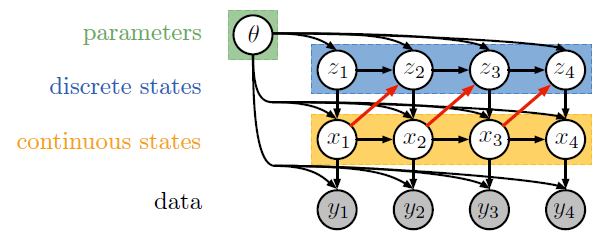
\includegraphics[width=0.5\textwidth]{rSLDS_diagram.png}
	\caption{The black arrows represent the dependencies of a tradidional SLDS, and the red arrows represent the added dependencies of an rSLDS.}
	\label{rSLDS}
\end{figure}

\textcolor{blue}{be aware, the stickbreaking is here!}

In the proposed model in the paper, the generation of discrete states $z_{t}$ follows:
$$
\begin{aligned}
z_{t+1} \mid z_{t}, x_{t},\left\{R_{k}, r_{k}\right\} & \sim \pi_{\mathrm{SB}}\left(\nu_{t+1}\right), \\
\nu_{t+1} & =R_{z_{t}} x_{t}+r_{z_{t}},
\end{aligned}
$$

where $R_{k} \in \mathbb{R}^{K-1 \times M}$ represents a weight matrix that specifies the recurrent dependencies, and $r_{k} \in \mathbb{R}^{K-1}$ is a bias that captures the Markov dependence of $z_{t+1}$ on $z_{t}$. The function $\pi_{\mathrm{SB}}: \mathbb{R}^{K-1} \rightarrow[0,1]^{K}$ maps a real vector to a normalized probability vector using the stick-breaking process, defined as follows:
$$
\begin{gathered}
\pi_{\mathrm{SB}}(\nu)=\left(\begin{array}{lll}
\pi_{\mathrm{SB}}^{(1)}(\nu) & \cdots & \pi_{\mathrm{SB}}^{(K)}(\nu)
\end{array}\right), \\
\pi_{\mathrm{SB}}^{(k)}(\nu)=\sigma\left(\nu_{k}\right) \prod_{j<k}\left(1-\sigma\left(\nu_{j}\right)\right)=\sigma\left(\nu_{k}\right) \prod_{j<k} \sigma\left(-\nu_{j}\right),
\end{gathered}
$$
for $k=1,2, \ldots, K-1$ and $\pi_{\mathrm{SB}}^{(K)}(\nu)=\prod_{k=1}^{K} \sigma\left(-\nu_{k}\right)$, where $\sigma(x)=e^{x} /\left(1+e^{x}\right)$ denotes the logistic function. The rest of the generative process of the rSLDS follows that of the SLDS. 

\subsection{Fitting rSLDSs} 
%%%%%%%%%%%%%%%%%%%%%%%%%%%%%%%%%%%%%%%%%%
%%%%%%%%%%%%%%%%%%%%%%%%%%%%%%%%%%%%%%%%%%
%%%%%%%%%%%%%%%%%%%%%%%%%%%%%%%%%%%%%%%%%%
%%%%%%%%%%%%%%%%%%%%%%%%%%%%%%%%%%%%%%%%%%
%%%%%%%%%%%%%BELOW%%%%%%%%%%%%%%%%%%%%%%%%
%%%%%%%%%%%%%%%%%%%%%%%%%%%%%%%%%%%%%%%%%%
%%%%%%%%%%%%%%%%%%%%%%%%%%%%%%%%%%%%%%%%%%
%%%%%%%%%%%%%%%%%%%%%%%%%%%%%%%%%%%%%%%%%%
%%%%%%%%%%%%%%%%%%%%%%%%%%%%%%%%%%%%%%%%%%
Similar to SLDS, The fitting process of rSLDS is based on the Gibbs sampler. However, during the message passing stage, the message from time $t$ to time $t+1$, denoted $m_{t \rightarrow t+1}\left(x_{t+1}\right)$, is computed via

$$
\int \psi\left(x_{t}, y_{t}\right) \psi\left(x_{t}, z_{t+1}\right) \psi\left(x_{t}, x_{t+1}, z_{t+1}\right) m_{t-1 \rightarrow t}\left(x_{t}\right) \mathrm{d} x_{t}
$$ 
where the inclusion of $\psi\left(x_{t}, z_{t+1}\right)$ accounts for the introduced dependence of $z_{t+1}$ on $x_t$.

With the previously defined stick-breaking function, one can derive the probability mass function $p(z \mid x)=\prod_{k=1}^{K} \sigma\left(\nu_{k}\right)^{\mathbb{I}[z=k]} \sigma\left(-\nu_{k}\right)^{\mathbb{[}[z>k]}
$, where $\mathbb{I}[\cdot]$ denotes an indicator function that takes value 1 when its argument is true and 0 otherwise. Therefore, the conditional distribution is non-Gaussian and the potential $\psi\left(x_{t}, z_{t+1}\right)$ is not a linear Gaussian factor. Thus, the integral in the message computation is not available in closed form, which makes the sampling of the latent continuous states challenging. In this paper, the Polya-gamma augmentation (\textcolor{red}{cite the polya-gamma trick here}) is used, which introduces an auxiliary variable.

According to the stick breaking mapping, the non-Gaussian factor is
$$\psi\left(x_{t}, z_{t+1}\right)=\prod_{k=1}^{K} \sigma\left(\nu_{t+1, k}\right)^{\mathbb{I}\left[z_{t+1}=k\right]} \sigma\left(-\nu_{t+1, k}\right)^{\mathbb{[}\left[z_{t+1}>k\right]}$$ where  $\nu_{t+1}$ is linear in $x_{t}$, and $\nu_{t+1, k}$ is the $k$-th dimension of $\nu_{t+1}$.  Expanding the definition of the logistic function, we have
$$
\psi\left(x_{t}, z_{t+1}\right)=\prod_{k=1}^{K-1} \frac{\left(e^{\nu_{t+1, k}}\right)^{\mathbb{I}\left[z_{t+1}=k\right]}}{\left(1+e^{\nu_{t+1, k}}\right)^{\mathbb{I}\left[z_{t+1} \geq k\right]}} \quad (*)
$$
An integral identity exists for polya-gamma distribution, given by:
$$
\frac{\left(e^{\nu}\right)^{a}}{\left(1+e^{\nu}\right)^{b}}=2^{-b} e^{\kappa \nu} \int_{0}^{\infty} e^{-\omega \nu^{2} / 2} p_{\mathrm{PG}}(\omega \mid b, 0) \mathrm{d} \omega \quad(**)
$$
where $\kappa=a-b / 2$ and $p_{\mathrm{PG}}(\omega \mid b, 0)$ is the density of the Pólya-gamma distribution, PG $(b, 0)$, which does not depend on $\nu$.   

Notice that the right hand side of (**) exhibits the same form of the left hand side of (*), while the right hand side of (*) can be viewed as an integral of a joint density $e^{-\omega \nu^{2} / 2} p_{\mathrm{PG}}(\omega \mid b, 0)$. Moreover, if we can represent this joint density as a factorized expression with $p_{\mathrm{PG}}(\omega \mid b, 0)$, the resulting factor will adopt the form $e^{-\omega \nu^{2} / 2}$, enabling manipulation into a Gaussian distribution. This observation inspires us to 
express  $\psi\left(x_{t}, z_{t+1}\right)$ as a marginal of $\psi\left(x_{t}, z_{t+1}, \omega \right)$, which is a factor defined on the augmented space, $\psi\left(x_{t}, z_{t+1}, \omega_{t}\right)$, where $\omega_{t} \in \mathbb{R}_{+}^{K-1}$ is a vector of auxiliary variables. In particular, we choose the auxiliary variables as $\prob(\omega_{t, k} \mid x_{t}, z_{t+1}) \sim \mathrm{PG}\left(\mathbb{I}\left[z_{t+1} \geq k\right], \nu_{t+1, k}\right)$. Then,  we have $\psi\left(x_{t}, z_{t+1}, \omega_{t}\right) \propto \prod_{k=1}^{K-1} \exp \left\{\kappa_{t+1, k} \nu_{t+1, k}-\frac{1}{2} \omega_{t, k} \nu_{t+1, k}^{2}\right\}$, where $\kappa_{t+1, k}=\mathbb{I}\left[z_{t+1}=k\right]-\frac{1}{2} \mathbb{I}\left[z_{t+1} \geq k\right]$. Recalling that $\nu_{t+1}$ is a linear function of $x_{t}$, 
$$
\psi\left(x_{t}, z_{t+1}, \omega_{t}\right) \propto \mathcal{N}\left(\nu_{t+1} \mid \Omega_{t}^{-1} \kappa_{t+1}, \Omega_{t}^{-1}\right),
$$
with $\Omega_{t}=\operatorname{diag}\left(\omega_{t}\right)$ and $\kappa_{t+1}=\left[\kappa_{t+1,1} \ldots, \kappa_{t+1, K-1}\right]$. 

Thus, after augmentation, the potentials on $x_{t}$ becomes Gaussian, allowing the integrals required for message passing to be written analytically. As a result, the Gibbs sampling of $\{x_t\}_{t=1:T}$ can be performed efficiently. Meanwhile, in each iteration of Gibbs sampling, an additional step is needed to sample the auxiliary variables by $\omega_{t, k} \mid x_{t}, z_{t+1} \sim \mathrm{PG}\left(\mathbb{I}\left[z_{t+1} \geq k\right], \nu_{t+1, k}\right)$. Finally, the recurrence weights, which are introduced to model the dependence of $z$ on $x$, are also conjugate under a MNIW prior, given the auxiliary variables $\omega_{1: T}$. This conjugate pair ensures the efficient sampling of the paramters $\theta$.

%%%%%%%%%%%%%%%%%%%%%%%%%%%%%%%%%%%%%%%%%%
%%%%%%%%%%%%%%%%%%%%%%%%%%%%%%%%%%%%%%%%%%
%%%%%%%%%%%%%%%%%%%%%%%%%%%%%%%%%%%%%%%%%%
%%%%%%%%%%%%%%%%%%%%%%%%%%%%%%%%%%%%%%%%%%
%%%%%%%%%%%%%ABOVE%%%%%%%%%%%%%%%%%%%%%%%%
%%%%%%%%%%%%%%%%%%%%%%%%%%%%%%%%%%%%%%%%%%
%%%%%%%%%%%%%%%%%%%%%%%%%%%%%%%%%%%%%%%%%%
%%%%%%%%%%%%%%%%%%%%%%%%%%%%%%%%%%%%%%%%%%
%%%%%%%%%%%%%%%%%%%%%%%%%%%%%%%%%%%%%%%%%%


\subsection{Conclusions from the Paper}

In the paper (\textcolor{red}{Cite Linderman Here}), the authors use three examples to demonstrate the capabilities (and limitations) of SLDSs and rSLDSs. These examples are data produced by an actual rSLDS (Synthetic NASCAR), data simulated from a well-studied classical dynamical system (Lorenz Attractor), and real data (Basketball Player Trajectories).

The models performed reasonably well on the synthetic data. Figure \ref{trueNascar} shows the true latent dynamics of the synthetic NASCAR simulation.
\begin{figure}[h!]
	\centering
	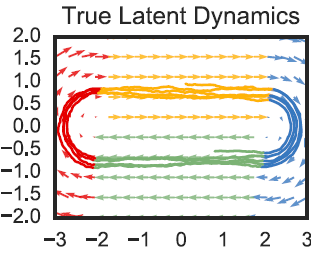
\includegraphics[width=0.35\textwidth]{paper_fig1.png}
	\caption{True dynamics of synthetic NASCAR}
	\label{trueNascar}
\end{figure}

Figure \ref{Nascargen} shows the states generated by both the SLDS and rSLDS fitting of the data. We can see that the rSLDS far outperformed the SLDS. This makes sense because the data was actually generated from an rSLDS, which the SLDS model will not be able to capture. Although this is just simulated data, this proof of concept demonstrates that if the data does indeed come from an SLDS or rSLDS, the approach from the paper will generate a reasonable interpretation of that data.

\begin{figure}[h!]
	\centering
	\begin{subfigure}[b]{0.35\textwidth}
		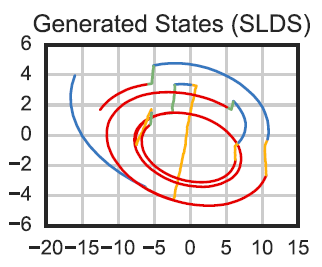
\includegraphics[width=\textwidth]{paper_fig3.png}
		\caption{SLDS}
	\end{subfigure}
	\begin{subfigure}[b]{0.35\textwidth}
		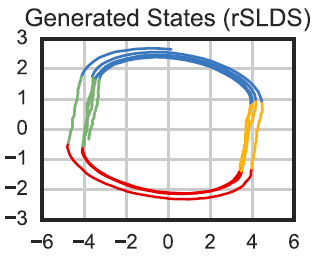
\includegraphics[width=\textwidth]{paper_fig4.png}
		\caption{rSLDS}
	\end{subfigure}
	\caption{Generated states of fit data for synthetic NASCAR}
	\label{Nascargen}
\end{figure}

The next example the authors considered was a system generated by the Lorenz system, a classical nonlinear dynamical system that exhibits chaotic dynamics, switching between two distinct states. However, rather than using Gaussian observations as in a traditional rSLDS, the authors of the paper apply a generalized linear model to the simulated time series data generated by the differential equations and then apply the logistic function. Finally, they collect 100 Bernoulli observations to use as the data to fit the model on.

\begin{figure}[h!]
	\centering
	\begin{subfigure}[b]{0.35\textwidth}
		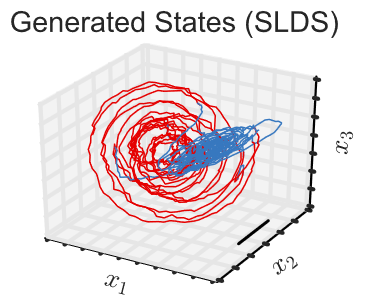
\includegraphics[width=\textwidth]{paper_fig5.png}
		\caption{SLDS}
	\end{subfigure}
	\begin{subfigure}[b]{0.35\textwidth}
		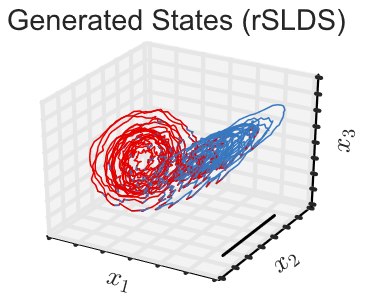
\includegraphics[width=\textwidth]{paper_fig6.png}
		\caption{rSLDS}
	\end{subfigure}
	\caption{Generated states of fit data for the Lorenz data}
	\label{Lorenzgen}
\end{figure}

We can see in Figure \ref{Lorenzgen} that both the SLDS model and the rSLDS model perform reasonably well. The authors found that the rSLDS did perform slightly better than the standard SLDS.

Finally, the authors analyzed data from real basketball players. The data used to fit the model were trajectories from five players in an NBA game between the Miami Heat and the Brooklyn Nets. Rather than an rSLDS, the authors fit the data to a recurrent autoregressive HMM (rAR-HMM), another generalization of the SLDS, where instead of passing through observations of the underlying continuous states, the continuous states are observed directly. These states are assumed to be generated by $K$ latent discrete states. The authors present a subset of these states, and labels them with names of basketball plays that they appear to represent. When comparing these states against those created by a random walk, the predicted states from the recurrent model perform far better; however, there is not evidence that the predicted states capture meaningful patterns in the movements of the players better than the random walk.

\subsection{New Methods}

To reproduce the results of the paper and to apply the models to more systems, we used a more up-to-date approach, as presented in (\textcolor{red}{Cite Blei Paper and Zoltowski paper}). These approaches are Black Box Variational Inference (BBVI) and Laplace Variational EM. These models are called state space models (SSMs).

The first approach is based on variational inference, a method from machine learning that approximates probability densities through optimization. The general idea of this approach is to first propose a family of densities that the target data may arise from and find one that generates data close to the target. The "black box" component of this approach is in reference to a class of these models that avoids any model-specific derivations, so that they can be used for a wide variety of problems. The latter approach combines variational and Laplace approximations over the underlying discrete and continuous variables.

